

%!TEX root = ../dissertation.tex
\chapter{FUNCTIONAL DATA ANALYSIS OF SATELLITE MEASUREMENTS OF PHENOLOGICAL PROCESSES} \label{future work}

\section{Introduction}

Phenology is the study of annual life-cycles of terrestrial vegetation and how they are effected by climate change or other environmental variables. Understanding vegetation phenology and its spatio-temporal variation is required to reveal and predict ongoing changes in Earth system dynamics \cite{Jeganathan:2010:0921-2973:1125}. The goal of this work is to develop a flexible model for vegetation life-cycles. A single life-cycle is determined by two variables: onset of greenness (OG) and end of senescence (ES). Figure \ref{fig:phenology diagram} illustrates how these values are defined. We use Multi-temporal Medium Resolution Imaging Spectrometer (MERIS) Terrestrial Chlorophyll Index (MTCI) data to derive onset of greenness and end of senescence for major tropical vegetation types.

\section{Initial Exploratory Work} We have only recently started working with this data set. As an initial step we have chosen a subset of the data corresponding to the $10\time 10$ grid shown in Figure \ref{fig:land use map}. The first year of data for these locations are shown in Figure \ref{fig:region6 curves}, with colors indicating the four different land cover types in the subset. Using these data the nonparametric covariance estimator described in Chapter \ref{ch:covariance estimation} was used to estimate the covariance function and corresponding eigenfunctions. The first five eigenfunctions shown in Figure \ref{fig:basis functions} were used as basis functions producing the fitted curves shown in Figure \ref{fig:estimated curves}. 

In order to understand the type of variation represented by an eigenfunction \cite{FDA} recommend adding and subtracting the eigenfunction from the mean function. Plots of this type are shown in Figure \ref{fig:interpreting eigenfunctions}. Notice how the second eigenfunction explains variation in the concavity of the function at the beginning of the season. The difference between tropical evergreen vegetation and coastal vegetation can largely be explained by the values of the coefficients for the second eigenfunction (see Figure \ref{fig:histogram coefs}). The total variation in coefficient values for all basis functions are shown in Figure \ref{fig:coef boxplot} illustrating how the majority of the variation is explained with only the first few eigenfunctions. 
\begin{figure}[htbp] 
	\centering 
	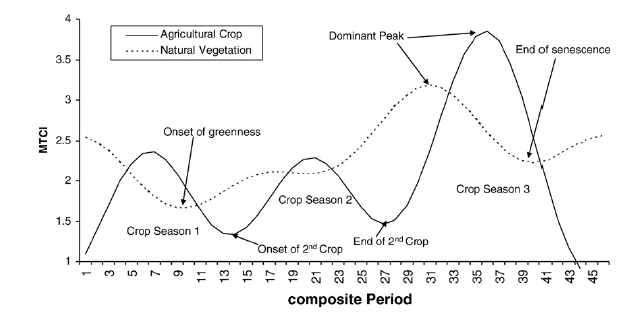
\includegraphics[width=\linewidth]{Images-phenology-fda/Plots/PhenoVars_Jegan.png} \caption{Diagram illustrating typical phenology patterns for agricultural land and natural vegetation. } \label{fig:phenology diagram} 
\end{figure}


